A typical workflow of a scientist who writes a scientific publication is to use a \gls*{wp} to write the paper and one or more \gls*{cas} for verification, analysis and visualization. Especially in \gls*{stem} literature, \LaTeX\footnote{Note that technically \LaTeX{} is not a \gls*{wp} (\url{https://www.latex-project.org/about/}, seen 07/2017) like \textit{Microsoft Word}. However, since \LaTeX{} (an extension of \TeX) is the standard to write articles in \gls*{stem} and we only focus on mathematical writings in this paper, we categorize \LaTeX{} as a \gls*{wp} as well.} has become the de facto standard for writing scientific publications over the past 30 years~\parencites{LATEX:Standard}[559]{DigitalTypo}{Knuth}. \LaTeX{} enables printing of mathematical formulae in a structure similar to handwritten style. For example, consider the Jacobi polynomial~\parencite[18.3 in table 1]{NIST:DLMF}
\begin{equation}\label{eq:P}
P_n^{(\alpha , \beta)}(\cos(a\Theta)),
\end{equation}
where $\alpha, \beta > -1$, and $n$ a nonnegative integer. 
This formula is written in \LaTeX{} as
\begin{equation*}
\verb|P_n^{(\alpha,\beta)}(\cos(a\Theta))|.
\end{equation*}

While \LaTeX{} focuses on displaying mathematics, a \gls*{cas} concentrates on computations and user friendly syntax. Especially important for a CAS is to embed unambiguous semantic information within the input. Each system uses different representations and syntax in consequence. Hence, a writer needs to constantly translate mathematical expressions from one representation to another and back again. Table~\ref{tab:JacobiP-usecase} shows four different representations for the same formula~(\ref{eq:P}).

\begin{table}[ht]
	\centering
	\begin{tabular}{ll}
		\hline
		Systems & Representations \\
		\hline
		\hline
		Generic \LaTeX\ & \verb|P_n^{(\alpha,\beta)}(\cos(a\Theta))| \\ 
		Semantic \LaTeX\ & \verb|\JacobiP{\alpha}{\beta}{n}@{\cos@{a\Theta}}| \\
		\Maple & \verb|JacobiP(n,alpha,beta,cos(a*Theta))| \\ 
		\Mathematica & \verb|JacobiP[n,\[Alpha],\[Beta],Cos[a \[CapitalTheta]]]|\\
		\hline
	\end{tabular}
	\caption{Different representations for the same mathematical formula~(\ref{eq:P}). Generic \LaTeX{} is the default \LaTeX{} expression. Semantic \LaTeX{} uses special semantic macros to embed semantic information.}
	\label{tab:JacobiP-usecase}
\end{table}

Translations from generic \LaTeX{} to \gls*{cas} are difficult to realize since the semantic information is not explicitly given in the input. The \gls*{nist} has created a set of semantic \LaTeX{} macros~\cite{DLMF:Macros}. Each macro ties specific character sequences to a well-defined mathematical object and is linked with the corresponding definition in the \gls*{dlmf} or \gls*{drmf}. These macros embed necessary semantic information into \LaTeX{} expressions. One example of such a macro is given table~\ref{tab:JacobiP-usecase} for the semantic \LaTeX{} representation for the Jacobi polynomial. The macros provide isolated access to important parts of the mathematical function, such as the arguments. 

Even with embedded semantic information, a translation between the systems can be difficult. A typical example of complex problems occurs for multivalued functions~\parencite{AISC:MultivaluedFunctions}. A \gls*{cas} usually defines \textit{branch cuts} to compute principal values of multivalued functions~\parencite{Maple:Cuts}, which makes the implementation of a theoretically continues function to a discontinued presentation of it. In general, positioning branch cuts follows conventions, but can be positioned arbitrarily in many cases. Communicate and explain the decision of defined branch cuts is a critical point for \gls*{cas} and can vary between the systems~\parencite{Branches:acot}. Figure~\ref{fig:acot-cut-compare} illustrates two examples of different branch cut positioning for the inverse trigonometric arccotangent function. While \Maple{} defines the branch cut at ${[-\infty\iunit, -\iunit]}$, ${[\iunit,\infty\iunit]}$ (figure~\ref{fig:acot-cut1}), \Mathematica{} defines the branch cut at ${[-\iunit, \iunit]}$ (figure~\ref{fig:acot-cut2}).

\begin{figure}[ht]
    \centering
    \subfloat[The real part of arccotangent with a branch cut at ${[-\infty\iunit, -\iunit]}$, ${[\iunit,\infty\iunit]}$.]{%
        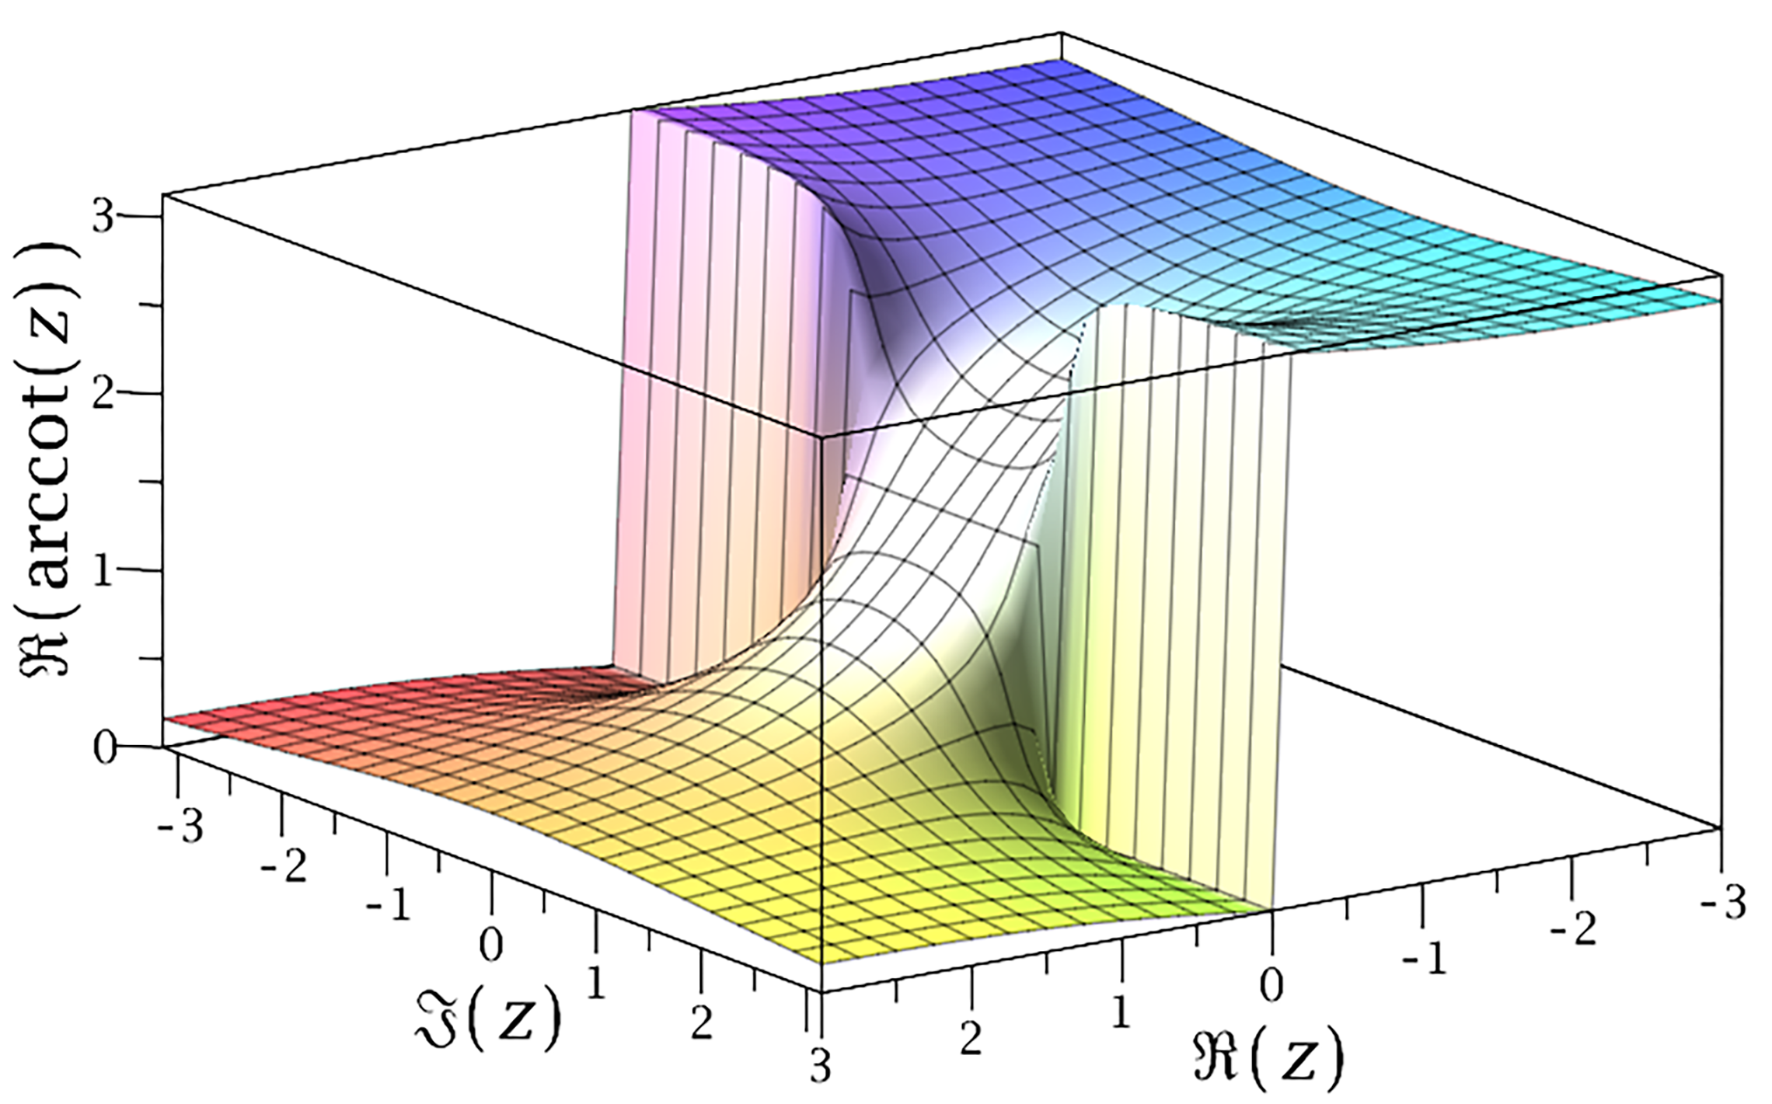
\includegraphics[width=0.45\textwidth]{acotCut1.png}
        \label{fig:acot-cut1}%
    }
    \hspace{0.5cm}
    \subfloat[The real part of arccotangent with a branch cut at ${[-\iunit, \iunit]}$.]{%
        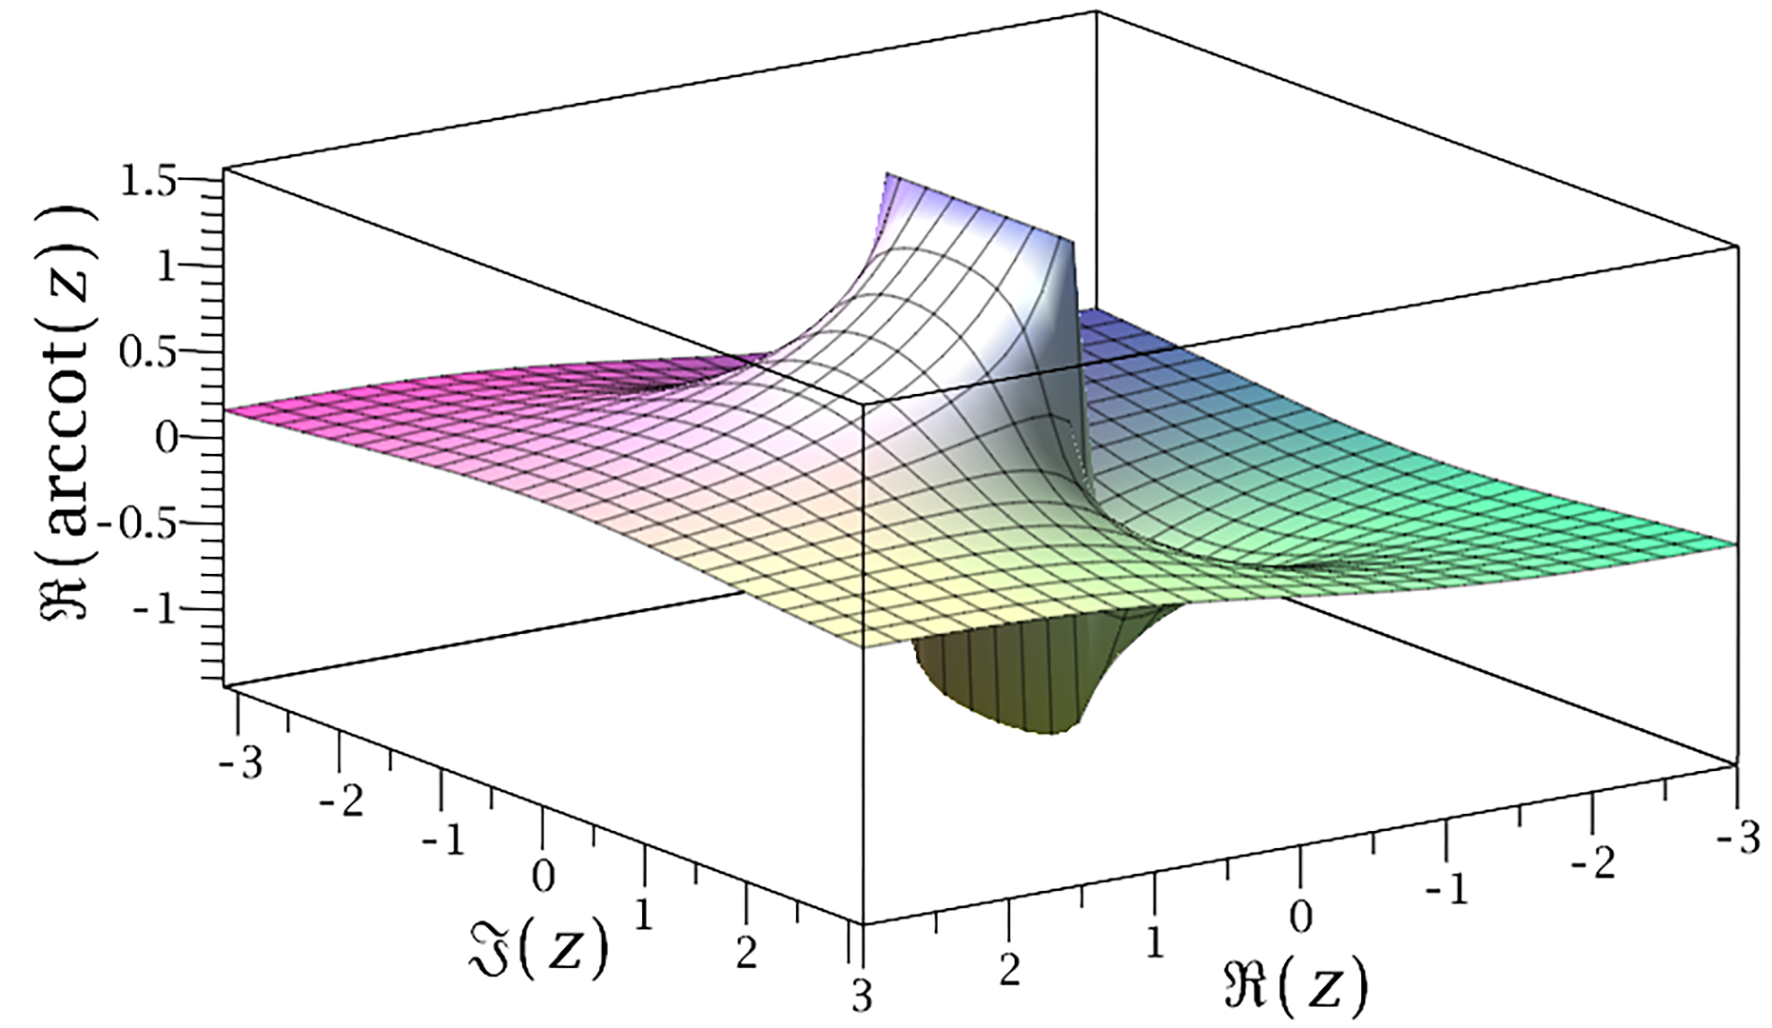
\includegraphics[width=0.45\textwidth]{acotCut2.png}
        \label{fig:acot-cut2}%
    }
    \caption{Two plots for the real part of the arccotangent function with a branch cut at $[-\infty\iunit, -\iunit]$, $[\iunit,\infty\iunit]$ in figure~\protect\subref{fig:acot-cut1} and at $[-\iunit, \iunit]$ in figure~\protect\subref{fig:acot-cut2}, respectively. (Plotted with \Maple{} 2016)}
    \label{fig:acot-cut-compare}
\end{figure}

Hence, a \gls*{cas} user needs to fully understand the properties and special definitions (such as the position of branch cuts) in the \gls*{cas} to avoid mistakes during a translation~\parencite{Maple:Cuts}. In consequence, a manual translation process is not only laborious, but also prone to errors. Note that this general problem has been named to automatic \gls*{p2c} conversion~\parencite{POM-Tagger}.

This article presents a new approach for automatic \gls*{p2c} and vice versa conversions. Translations from presentational to computational (computational to presentational) systems are called forward (backward) translations. A forward translation is denoted with an arrow with the target system language above the arrow. For example,
\begin{equation*}
t \overset{\langMaple}{\mapsto} c,
\end{equation*}
where $t$ is an expression in the \LaTeX{} language and $c$ is an element of the \Maple{} language $\langMaple$. As we will see later in this article, we need to compare mathematical concepts between systems. This is impossible from a mathematical point of view. Consider the irrational mathematical constant $e$, known as Euler's number. The theoretical construct for this symbol cannot be mathematically equivalent to the value \verb|exp(0)| in \Maple, caused by computational and implementational limitations. Instead of using the term \textit{equivalent}, we introduce a \textit{appropriate} and \textit{inappropriate} translations. We call a translation such as
\begin{equation}\label{eq:cos-def}
\verb|\cos@{z}| \overset{\langMaple}{\mapsto} \verb|cos(z)|
\end{equation}
as \textit{appropriate}, while a translation such as
\begin{equation}
\verb|\cos@{z}| \overset{\langMaple}{\mapsto} \verb|sin(z)|
\end{equation}
is called \textit{inappropriate}. Note that it is not always as easy as in this example to decide if a translation is appropriate or not. Therefore, this article also presents several validation techniques to automatically verify if a translation is appropriate or inappropriate. In addition to this terminology, we introduce \textit{direct translations}. Later in the paper, we will explain that a translation from one specific mathematical object to its \textit{appropriate} counterpart in the other system is not always possible. We call a translation to the \textit{appropriate} counterpart \textit{direct}. For example, the translation~(\ref{eq:cos-def}) is \textit{direct}, while a translation to the definition of the cosine function
\begin{equation*}
\verb|\cos@{z}| \overset{\langMaple}{\mapsto} \verb|(exp(I*z)+exp(-I*z))/2|
\end{equation*}
is not a \textit{direct} translation.

Note that partial results of this paper have been published in~\parencite{CICM:Paper}.
